\subsection{Prof. Dr. Andreas Bausch}


\textbf{Main Research Interests}\\[-0.25cm]
\begin{enumerate}
\item[$\bullet$]	Strategic Management
\item[$\bullet$]	International Management
\item[$\bullet$]  Controlling
\item[$\bullet$]	Entrepreneurship
\end{enumerate}


\vspace{0.6cm}
\textbf{Research Activities}\\[-0.25cm]

Prof. Bausch's major research focus has been on evidence-based best practices in strategic management and is anchored in the Center for Management Studies (CMS) at IUB. With the explosion of information from empirical research over the past decades, evidence-based strategic management strives to synthesize and interpret the research findings available in the field. Meta-analysis is to date widely used almost exclusively in medicine and psychology, having set a benchmark there. In the CMS meta-analysis is used to generate theory, to identify emerging issues in the field, to examine controversial or complicated topics, and to explicate "how to" strategies for practitioners. So far, internationalization, innovation, diversification, alliance activities, and mergers and acquisitions have been found to have a significant impact on firm performance.
\begin{figure}[ht]
  \begin{center}
    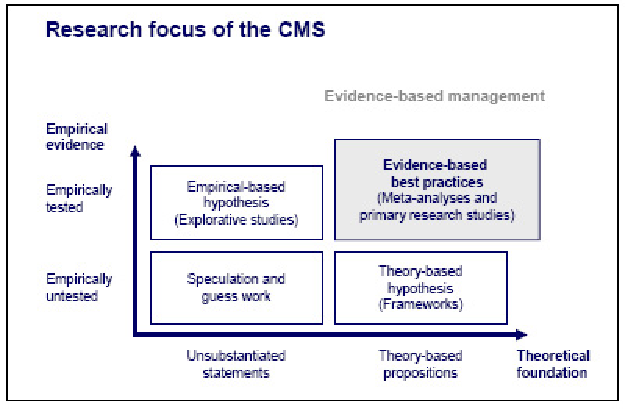
\includegraphics[width=0.7\linewidth]{./SocSci/Bausch-fig001.pdf}
%   \mycaption{ xxx )}\label{fig:profxxx}
   \end{center}
\end{figure}\\[-0.4cm]
After the success of the first two "Value Creator" studies (published in 2002 and 2004), a third study has been initiated together with Accenture. This study investigates the critical success factors of energy suppliers in Germany, Austria and Switzerland. In addition to accounting data from 1999 to 2005, this follow-up study will also be based on a management survey distributed to executives of utility companies. Together with The Advisory House AG a joint research funded by RWE AG analyzing demographic change in Europe and its impact on the labor market has been set-up. The overall aim of the study is not only to forecast the labor market in 2020 but also to develop comprehensive scenarios and to derive scenario specific recommendations for multinational corporations. Additionally, Prof. Andreas Bausch has submitted a research grant proposal on the antecedents and outcomes of radical vs. incremental innovation to the VolkswagenStiftung together with Profs. Michael Frese (Justus-Liebig-Universit�t Gie�en), James L. Farr (Penn State University), Shaker Zahra (University of Minnesota). The research team is planning to conduct a cross-cultural study on the influences of institutional, organizational, and psychological factors influencing radical and incremental innovation activity of firms in Germany and the US. 

\vspace{0.6cm}


\textbf{Funded Projects}\\[-0.25cm]
\begin{enumerate}
\item[$\bullet$]   Center for Management Studies - funded by The Advisory House AG
\item[$\bullet$]	 Empirical study "Value Creator III" - funded by Accenture GmbH
\item[$\bullet$]	 Empirical study "Demographic Change" - funded by RWE AG
\end{enumerate}


\vspace{0.6cm}
\textbf{Organization of Scientific Conferences}\\[-0.25cm]
\begin{enumerate}
\item[$\bullet$]	October 2006\newline
	Universit�t Bremen\newline
  "Unternehmertage 2006 - Der Mittelstand auf dem Weg ins Ausland"\newline
	funded by: PriceWaterhouseCoopers, Bremische Volksbank eG, 	Deutsche Bank, Bremer Landesbank, Commerzbank, Sparkasse 	Bremen 
\end{enumerate}


\vspace{0.6cm}
\textbf{Other Professional Activities}\\[-0.25cm]
\begin{enumerate}
\item[$\bullet$] Chair of Business Administration and International Management, School of Management and Economics, Friedrich Schiller Universit\"at Jena
\item[$\bullet$] Visiting Professor, Freie Universit\"at Bozen, Italy
\item[$\bullet$]	Academic Director of the Executive MBA Program in European Utility Management, International University Bremen
\item[$\bullet$]	Teaching of non-degree executive programs: amongst others for Deutsche Telekom, E.ON Academy, Salzgitter, and Delton
\end{enumerate}


\vspace{0.6cm}
\textbf{PhD-Students}\\[-0.25cm]

Kathrin B�secke\newline
\textit{Success Factors of Business Combinations}\\[-0.15cm]

Thomas Fritz\newline
\textit{Creating Superior Economic Performance through Sustainable Competitive Advantage}\\[-0.15cm]

Christian Grube\newline
\textit{The Valuation of Knowledge and Patents}\\[-0.15cm]

Mario Krist\newline
\textit{The Role of Intangible Resources in the Internationalization Process and their Contribution to Firm Performance}\\[-0.15cm]

Frithjof Pils\newline
\textit{Product Diversification and Corporate Financial Performance}\\[-0.15cm]

Nina Rosenbusch\newline
\textit{Antecedents and Outcomes of Radical vs. Incremental Innovation}\\[-0.15cm]

Duc Linh Van Tri\newline
\textit{Internationalization into the Chinese Market}



\vspace{0.6cm}
\textbf{Research Personnel}\\[-0.25cm]

Thomas Fritz\\[-0.15cm]

Duc Linh Van Tri
